% BEGIN LICENSE BLOCK
% Version: CMPL 1.1
%
% The contents of this file are subject to the Cisco-style Mozilla Public
% License Version 1.1 (the "License"); you may not use this file except
% in compliance with the License.  You may obtain a copy of the License
% at www.eclipse-clp.org/license.
% 
% Software distributed under the License is distributed on an "AS IS"
% basis, WITHOUT WARRANTY OF ANY KIND, either express or implied.  See
% the License for the specific language governing rights and limitations
% under the License. 
% 
% The Original Code is  The ECLiPSe Constraint Logic Programming System. 
% The Initial Developer of the Original Code is  Cisco Systems, Inc. 
% Portions created by the Initial Developer are
% Copyright (C) 2006 Cisco Systems, Inc.  All Rights Reserved.
% 
% Contributor(s): 
% 
% END LICENSE BLOCK

\chapter{Building Hybrid Algorithms}
\label{chaphybrid}
%HEVEA\cutdef[1]{section}

\section{Combining Domains and Linear Constraints}
Most optimisation problems arising in industry and commerce involve
different subproblems that are best addressed by different algorithms
and constraint solvers. In \eclipse{} it is easy to use different
constraint solvers in combination.  The different solvers may share
variables and even constraints.

We discuss reasons for combining the {\tt eplex} and {\em
IC} solver libraries and explore ways of doing this.  The {\tt repair}
library plays a useful role in propagating solutions generated by a
linear solver to other variables handled by the domain solver.
We show how this works in a generic hybrid algorithm termed {\em
probing}.

\section{Reasons for Combining Solvers}
The {\tt ic} solver library implements two kinds of constraints
\begin{itemize}
\item finite domain constraints
\item interval constraints
\end{itemize}
Each constraint is handled separately and individually, and the only
communication between them is via the bounds on their shared
variables. 

The benefits of the {\tt ic} solvers are
\begin{enumerate}
\item the repeated tightening of guaranteed upper and lower bounds on the
variables
\item the application of tailored algorithms to standard subproblems
(encapsulated as global constraints)
\item the implementation of a very wide class of constraints
\end{enumerate}

The {\tt eplex} solver library implements two kinds of constraints
\begin{itemize}
\item linear numeric constraints
\item integrality constraints
\end{itemize}
The linear constraints are handled by a very powerful solver that
enforces {\em global} consistency on all the constraints.
%taking into
%account all the interactions between the different linear constraints.
%This is much more powerful than handling the constraints separately.
The integrality constraints are handled via a built-in search
mechanism.

The benefits of the {\tt eplex} solvers are
\begin{enumerate}
\item the enforcement of global consistency for linear constraints
\item the production of an optimal solution satisfying the linear constraints
\end{enumerate}

For some years researchers have sought to characterise the classes of
problems for which the different solvers are best suited.  
Problems involving only linear constraints are very well handled by
{\tt eplex}.
Problems involving disjunctions of constraints are often best
handled by {\tt ic}.
Often set covering problems are best handled by {\tt eplex} and
scheduling problems by {\tt ic}.
However in general there is no method to recognise for a new problem
which solver is best.

Luckily in \eclipse{} there is no need to choose a specific solver for each
problem, since it is possible to apply both solvers.  Moreover the
solvers communicate with each other, thus further speeding up constraint
solving.
The {\tt ic} solver communicates new tightened bounds to the 
{\tt eplex} solver.  These tightened bounds have typically been deduced
from non-linear constraints and thus the linear solver benefits from
information which would not otherwise have been available to it.
On the other hand the {\tt eplex} solver often detects inconsistencies
which would not have been detected by the {\tt ic} solvers.  Moreover
it returns a bound on the optimisation function which can be used by
the {\tt ic} constraints.  
Finally the optimal solution returned by {\tt eplex} to the
``relaxed'' problem
comprising just the linear constraints, can be used as a
search heuristic that can focus the {\tt ic} solver on the most
promising parts of the search space.

\quickref{Motivation}{
There are two main reasons for combining {\tt eplex} and {\tt ic} in
a hybrid algorithm
\begin{itemize}
\item {\tt ic} handles a wider class of constraints than {\tt eplex}
\item The solvers extract
different kinds of information from the constraints
\end{itemize}
}

\section{A Simple Example}

\subsection{Problem Definition}
We start with a simple example of linear constraints being posted to
{\tt eplex} and the other constraints being sent to {\tt ic}.

The example problem involves three tasks ({\em task1, task2, task3})
and a time point 
{\em time1}.  We enforce the following constraints:
\begin{itemize}
\item Exactly one of {\em task1} and {\em task2} overlaps with {\em
time1}
\item Both tasks {\em task1} and {\em task2} precede {\em task3}
\end{itemize}

\subsection{Program to Determine Satisfiability}
For this example we handle the first constraint using {\tt ic},
because it is not expressible as a conjunction of linear constraints,
and we handle the second pair of linear constraints using {\tt eplex}.

\Note{Note that since we use both solvers {\tt eplex} and {\tt ic} we
will explicitly module qualify all numeric constraints to avoid
ambiguity.}
 
\index{overlap}
Each task has a start time $Start$ and a duration $Duration$.  
We encode the (non-linear) overlap constraint in {\tt ic} thus:
\begin{code}
:- lib(ic).
overlap(Start,Duration,Time,Bool) :-
        % Bool is 1 if the task with start time Start and duration
        % Duration overlaps time point Time and 0 otherwise
       ic: (Bool #= ((Time $>= Start) and (Time $=< Start+Duration-1))).
\end{code}
The variable {\em Bool} takes the value $1$ if the task overlaps the
time point, and $0$ otherwise.  To enforce that only one task overlaps
the time point, the associated boolean variables must sum to $1$.

\index{before}
We encode the (linear) precedence constraint in {\tt eplex} thus:
\begin{code}
:- lib(eplex).
before(Start,Duration,Time) :-
        % the task with start time Start and duration Duration is
        % completed before time point Time
        eplex: (Start+Duration $=< Time).
\end{code}

To complete the program, we can give durations of $3$ and $5$ to {\em
task1} and {\em task2}, and have the linear solver minimise the start
time of {\em task3}:
\begin{code}
ic_constraints(Time,S1,S2,B1,B2) :-
        % exactly one of task 1 with duration 3 and task 2 with
        % duration 5 overlaps time point Time
        ic: ([S1,S2]::1..20),
        overlap(S1,3,Time,B1),
        overlap(S2,5,Time,B2),
        ic: (B1+B2 #= 1).

eplex_constraints(S1,S2,S3) :-
        % task 1 with duration 3 and task 2 with duration 5 are both
        % completed before the start time of task 3
        before(S1,3,S3),
        before(S2,5,S3).
 
hybrid1(Time, [S1,S2,S3], End) :-
        % give the eplex cost variable some default bounds
        ic:(End $:: -1.0Inf..1.0Inf),
        % we must give the start time of task 3 ic bounds in order to
        % suspend on changes to them
        ic: (S3::1..20),
        % setup the problem constraints
        ic_constraints(Time,S1,S2,B1,B2),
        % setup the eplex solver
        eplex_constraints(S1,S2,S3),
        eplex:eplex_solver_setup(min(S3),End,[sync_bounds(yes)],[ic:min,ic:max]),
        % label the variables occurring in ic constraints
        labeling([B1,B2,S1,S2]).

\end{code}
During the labeling of the boolean variables, the bounds on $S1$ and
$S2$ are tightened as a result of {\tt ic} propagation, which wakes
the linear solver, which has been set to trigger on ic bound changes ({\tt
  ic:min, ic:max}). Note that all variables occurring in the linear
solver must then have ic attributes.

The ic bounds are passed to the linear solver before
the problem is solved with the option {\tt sync_bounds(yes)}. The
linear solver derives a new lower bound for $End$.  In case this
exceeds its upper bound, the search fails and backtracks.

Using this method of bound communication the bounds for {\em all}
problem variables are retrieved from any bounds solvers before
resolving the linear problem. If however only a small number of variable
bounds have changed sufficiently to affect the relaxed solution
this will be inefficient.

Instead bound updates for individual variables and bound solvers may
be transferred to the linear solver separately. This may be achieved
(using the {\tt eplex} instance's {\tt ::/2}) either explicitly within
the search code or through demons attached to the appropriate solver
bound changes. 

Note that the optimisation performed by the linear
solver does not respect the {\tt ic} constraints, so a correct answer
can only be guaranteed once all the variables involved in {\tt ic}
constraints are instantiated.

Henceforth we will not explicitly show the loading of the {\tt ic} and
{\tt eplex} libraries.

\subsection{Program Performing Optimisation}
\index{hybrid optimization}
When different constraints are sent to {\tt ic} and to {\tt eplex},
the optimisation built into the linear solver must be combined with
the optimisation provided by the \eclipse{} {\em branch\_and\_bound}
library. 

The following program illustrates how to combine these optimisations:
\begin{code}
:- lib(branch_and_bound).

hybrid2(Time, [S1,S2,S3], End) :-
        % give the eplex cost variable some default bounds
        ic:(End $:: -1.0Inf..1.0Inf),
        % we must give the start time of task 3 ic bounds in order to
        % suspend on changes to them
        ic: (S3::1..20),
        % setup the problem constraints
        ic_constraints(Time,S1,S2,B1,B2),
        eplex_constraints(S1,S2,S3),
        % perform the optimisation
        both_opt(labeling([B1,B2,S1,S2]),min(S3),End).

both_opt(Search,Obj,Cost) :-
        % setup the eplex solver
        eplex:eplex_solver_setup(Obj,Cost,[sync_bounds(yes)],[ic:min,ic:max]),
        % minimize Cost by branch-and-bound
        minimize((Search,eplex_get(cost,Cost)),Cost).
\end{code}

\quickref{A Simple Example}{
A simple way to combine {\tt eplex} and {\tt ic} is to send the linear
constraints to {\tt eplex} and the other constraints to {\tt ic}.
The optimisation primitives must also be combined.
}

\section{Sending Constraints to Multiple Solvers}
\index{multiple solvers}
\subsection{Syntax and Motivation}
Because of the cooperation between solvers, it is often useful to send
constraints to multiple solvers.
A linear constraint, such as $X+2 \ge Y$, can be posted to {\tt eplex} by
the code \verb0eplex: (X+2 $>= Y)0.  The same constraint can be posted
to {\tt ic} by the code \verb0ic: (X+2 $>= Y)0.  
The constraint can be sent to both solvers by the code 
\begin{quote}\begin{verbatim}
   [ic,eplex]: (X+2 $>= Y)
\end{verbatim}\end{quote}

By sending constraints to both solvers, where possible, we can
improve search algorithms for solving constraint problems.
Through enhanced constraint reasoning at each node of the search tree
we can:
\begin{itemize}
\item prune the search tree, thus improving efficiency
\item render the algorithm less sensitive to search heuristics
\end{itemize}
The second advantage is a particular benefit of combining different
solvers, as opposed to enhancing the reasoning power of a single
solver. 
See \cite{RWH99} and \cite{rodosekcp} for
experimental results and application examples using multiple solvers
in this way. 

\subsection{Handling Booleans with Linear Constraints}
\index{disjunctive}
The \verb0overlap0 constraint example above is disjunctive and
therefore non-linear, and is only handled by {\tt ic}.
However as soon as the boolean variable is labelled to $1$, during
search, the constraint becomes linear.

The cooperation between the {\tt eplex} and {\tt ic} solvers could
therefore be improved by passing the resulting linear constraint to
{\tt eplex} as soon as the boolean is labelled to $1$.
This could be achieved using a constraint handling rule (see CHR) or a
suspended goal (see chapter \ref{chapimpl}).

\index{bigM transformation}
However the same improved cooperation can be achieved by a well known
mathematical programming technique (see e.g.\ \cite{Williams99})
that builds the boolean variable into a linear constraint that can be
sent to {\tt eplex} even before the boolean is instantiated. 
This linear constraint effectively enforces the {\em overlap}
constraint if the boolean is instantiated to $1$, but does not enforce
it if the boolean is instantiated to $0$.

To achieve this we introduce sufficiently big multipliers, that when
the boolean is set to $0$ the 
constraint is satisfied {\em for all values within the variables'
bounds}.
This method is known as the {\em bigM} transformation.

It is illustrated in the following encoding
of \verb0pos_overlap0:
\begin{code}
pos_overlap(Start,Duration,Time,Bool) :-
        % if Bool is 1 then the task with start time Start and
        % duration Duration overlaps time point Time
        Max1 is maxdiff(Start,Time),
        Max2 is maxdiff(Time,Start+Duration-1),      
        eplex: (Time+(1-Bool)*Max1 $>= Start),              % lin1
        eplex: (Time $=< Start+Duration-1+(1-Bool)*Max2).   % lin2

maxdiff(Expr1,Expr2,MaxDiff) :-
        % the maximum diffrence between Expr1 and Expr2 is the max val
        % of (Expr1 - Expr2)
        MaxDiff is max_val(Expr1 - Expr2).

max_val(Expr, Max) :-
        % the maximum value of a variable is its upper bound
        var(Expr),!,
        get_var_bounds(Expr, _, Max).
max_val(Expr, Max) :-
        % the maximum value of a number is itself
        number(Expr),!,
        Max = Expr.
max_val(Expr1 + Expr2, Max) :-
        % the maximum value of (Exrp1 + Expr2) is the maximum value of
        % Expr1 plus the maximum value of Expr2
        Max is max_val(Expr1) + max_val(Expr2).
max_val(Expr1 - Expr2, Max) :-
        % the maximum value of (Exrp1 - Expr2) is the maximum value of
        % Expr1 minus the minimum value of Expr2
        Max is max_val(Expr1) - min_val(Expr2).

min_val(Expr, Min) :-
        % the minimum value of a variable is its lower bound
        var(Expr),!,
        get_var_bounds(Expr, Min, _).
min_val(Expr, Min) :-
        % the minimum value of a number is itself
        number(Expr),!,
        Min = Expr.
min_val(Expr1 + Expr2, Max) :-
        % the minimum value of (Exrp1 + Expr2) is the minimum value of
        % Expr1 plus the minimum value of Expr2
        Max is min_val(Expr1) + min_val(Expr2).
min_val(Expr1 - Expr2, Max) :-
        % the minimum value of (Exrp1 - Expr2) is the minimum value of
        % Expr1 minus the maximum value of Expr2
        Max is min_val(Expr1) - max_val(Expr2).
\end{code}

The linear constraints, which will enforce the overlap condition when
the variable \verb0Bool0 is set to $1$, are labelled
{\em lin1} and {\em lin2}.
If the variable \verb0Bool0 is instantiated to $0$, then the variables (or
values) \verb0Start0, \verb0Time0 and \verb0Duration0 are free to take
any value in their respective domains.

\index{linear relaxation}
Notice that \verb0pos_overlap0 is logically weaker than \verb0overlap0
because 
\begin{itemize}
\item it does not enforce the integrality of the boolean variable,
(i.e. \verb0pos_overlap0 is a linear relaxation of the disjunctive
constraint), and
\item 
it does not enforce the negation of {\em overlap} in case the
boolean is set to $0$.
\end{itemize}

The tighter cooperation is achieved simply by adding the
\verb0pos_overlap0 constraint to the original encoding:
\begin{code}
eplex_constraints_2(Time,S1,S2,S3,B1,B2) :-
        % task 1 with duration 3 and task 2 with duration 5 are both
        % completed before the start time of task 3
        before(S1,3,S3),
        before(S2,5,S3),
        % task 1 with duration 3 overlaps time point Time if B1 = 1
        pos_overlap(S1,3,Time,B1),
        % task 2 with duration 5 overlaps time point Time if B2 = 1
        pos_overlap(S2,5,Time,B2).

hybrid3(Time, [S1,S2,S3], End) :-
        % give the eplex cost variable some default bounds
        ic:(End $:: -1.0Inf..1.0Inf),
        % we must give the start time of task 3 ic bounds in order to
        % suspend on changes to them
        ic: (S3::1..20),
        % setup the problem constraints
        ic_constraints(Time,S1,S2,B1,B2),
        eplex_constraints(Time,S1,S2,S3,B1,B2),
        % perform the optimisation
        both_opt(labeling([B1,B2,S1,S2]),min(S3),End).
\end{code}

Although it may at first glance seem better to enforce the
integerality of all variables in the linear solver as well, this is in
fact counter-productive for variables that will be explicitly labelled
during search in hybrid algorithms. The external solver would
then perform its own branch-and-bound search in addition to the
branch-and-bound search being performed within the \eclipse{} program.

\subsection{Handling Disjunctions}

The same technique, of introducing boolean variables and sufficiently
large multipliers, can be used to translate any disjunction of linear
constraints into linear constraints (and integrality constraints on
the booleans) which can be handled by {\tt eplex}.

Consider the negation of the {\em overlap} constraints above: if a task does
not overlap a time point then it is {\em either} completed before the
time point {\em or} starts after the timepoint. This disjunction can
be expressed in {\tt eplex} using two further boolean variables:
\begin{code}
neg_overlap(Start,Duration,Time,Bool1,Bool2) :-
        % if Bool1 is 1 then the task with start time Start and duration
        % Duration starts after time point Time
        Max1 is maxdiff(Time,Start-1),
        eplex:(Time $=< Start-1+(1-Bool1)*Max1),
        % if Bool2 is 1 then the task with start time Start and duration
        % Duration is completed before time point Time
        Max2 is maxdiff(Start+Duration,Time),
        eplex:(Time+(1-Bool2)*Max2 $>= Start+Duration).

eplex_constraints_3(T,S1,S2,S3,B1,N1B1,N2B1,B2,N1B2,N2B2) :-
        % task 1 with duration 3 and task 2 with duration 5 are both
        % completed before the start time of task 3
        before(S1,3,S3),
        before(S2,5,S3),
        % task 1 with duration 3 either overlaps time point Time,
        % starts after it or is completed before it
        pos_overlap(S1,3,T,B1),
        neg_overlap(S1,3,T,N1B1,N2B1),
        eplex:(N1B1+N2B1 $= 1-B1),
        % task 2 with duration 5 either overlaps time point Time,
        % starts after it or is completed before it
        pos_overlap(S2,5,T,B2),
        neg_overlap(S2,5,T,N1B2,N2B2),
        eplex:(N1B2+N2B2 $= 1-B2),
        % exactly one of task 1 with duration 3 and task 2 with
        % duration 5 overlaps time point Time
        eplex:(B1+B2 $= 1).

hybrid4(Time, [S1,S2,S3], End) :-
        % give the eplex cost variable some default bounds
        ic:(End $:: -1.0Inf..1.0Inf),
        % we must give the start time of task 3 and the non-overlap
        % booleans ic bounds in order to suspend on changes to them
        ic:(S3::1..20),
        ic:([N1B1,N2B1,N1B2,N2B2]::0..1),
        % setup the problem constraints
        ic_constraints(Time,S1,S2,B1,B2),
        eplex_constraints_3(Time,S1,S2,S3,B1,N1B1,N2B1,B2,N1B2,N2B2),
        % perform the optimisation
        both_opt(labeling([B1,N1B1,N2B1,B2,N1B2,N2B2,S1,S2]),min(S3),End).
\end{code}

Now the negation of the overlap will be enforced whenever either of
the non-overlap booleans is set to 1. Note that it is not strictly
necessary to label the non-overlap booleans: whenever the start time
of a task is labelled in such a way that the task falls to one side of
the time point, the other non-overlap boolean will be forced to 0
by its linear non-overlap constraint. The constraint requiring a task
to either overlap or fall to one side of the time point will then
force the remaining non-overlap boolean to be 1.

In fact in this simple example we gain nothing by including the {\tt
neg\_overlap} constraints on the ``direction'' of non-overlap. As soon
as a labeling decision has been made as to whether one task overlaps
the time point, the earliest possible start time of both tasks is
updated in the linear solver. Since the problem cost is minimized by
starting all tasks as early as possible, the relaxed {\tt eplex}
solution will conicide with the integer solution.

As another simple example consider a naive program to choose values for the
elements of a finite list (of length \verb0Length0) such that each
pair of values differs by at least $2$. 
The {\em diff2} constraint on each pair \verb0X0 and \verb0Y0 
of elements can be expressed as a disjunction in {\tt ic}:
\begin{code}
diff2ic(X,Y) :-
        % X and Y must differ by at least 2
        ic: ((X+2 $=< Y) or (Y+2 $=< X)).

list_diff2ic(List) :-
        % each pair must differ by at least 2
        (
            fromto(List, [X|Rest], Rest, [])
        do
            (
                foreach(Y, Rest),
                param(X)
            do
                diff2ic(X,Y)
            )
        ).
\end{code}
Alternatively it can be expressed in {\tt eplex} using a boolean
variable:
\begin{code}
diff2eplex(X,Y,Length,B) :-
        % if B is 1 then Y is at least 2 greater than X
        eplex: (X+2+B*Length $=< Y+Length),
        % if B is 0 then X is at least 2 greater than Y
        eplex: (X+Length $>= Y+2+(1-B)*Length).

list_diff2eplex(List, Length, Bools) :-
        % each pair must differ by at least 2
        (
            fromto(List, [X|Rest], Rest, []),
            fromto(Bools, Out, In, []),
            param(Length)
        do
            (
                foreach(Y, Rest),
                fromto(Out, [B|Bs], Bs, In),
                param(X, Length)
            do
                diff2eplex(X,Y,Length,B)
            )
        ).
\end{code}

Suppose each element $E$ of the list must
take a value between $1$ and $2*(Length-1)$, 
then any attempted labelling of the elements must fail.
Sending the constraints to {\tt ic} and labelling the elements of the
list is inefficient.
\begin{code}
ic_list(List) :-
        length(List, Length),
        Max is 2*(Length-1),
        % each element must take a value between 1 and 2*(Length-1)
        ic: (List::1..Max),
        list_diff2ic(List),
        labeling(List).
\end{code}

Sending the constraints to {\tt eplex} and enforcing integrality of
the booleans is more efficient.
\begin{code}
eplex_list(List) :-
        length(List, Length),
        Max is 2*(Length-1),
        % each element must take a value between 1 and 2*(Length-1)
        eplex: (List::1..Max),
        list_diff2eplex(List, Length, Bools),
        % enforce Bools to be 0..1 and integer
        eplex: integers(Bools),
        eplex: (Bools::0..1),
        % setup the eplex solver with a dummy objective function
        eplex:eplex_solver_setup(min(0),Cost,[],[]),
        % solve by linear solver
        eplex:eplex_solve(Cost).
\end{code}

Better still is to post the constraints to both {\tt ic} and 
{\tt eplex}, 
and label the booleans.
\begin{code}
hybrid_list(List) :-
        % give the eplex cost variable some default bounds
        ic:(Cost $:: -1.0Inf..1.0Inf),
        length(List, Length),
        Max is 2*(Length-1),
        % each element must take a value between 1 and 2*(Length-1)
        ic: (List::1..Max),
        list_diff2ic(List),
        list_diff2eplex(List, Length, Bools),
        % enforce Bools to be 0..1 (but not integer in eplex)
        ic: (Bools::0..1),
        % setup the eplex solver with a dummy objective function
        eplex:eplex_solver_setup(min(0),Cost,[sync_bounds(yes)],[ic:min,ic:max]),
        % minimize Cost by branch-and-bound
        minimize((labeling(Bools),eplex_get(cost,Cost)),Cost).
\end{code}

\subsection{A More Realistic Example}
\index{generating test networks}
For more complex applications, sending all ``linearisable''
constraints to both {\tt ic} and {\tt eplex} is rarely the best
method.
Sending too many constraints to {\tt ic} can result in many wakings
but little useful propagation.
Sending too many constraints to {\tt eplex} can cause a big growth
in the size of the constraint store, which slows down constraint
solving with little improvement in the relaxed optimum.
If the extra variables are constrained to be integer, then the (MIP)
solver may enter a deep search tree with disastrous consequences for
efficiency.
In this example we briefly illustrate the point, though there is no
space to include the whole program, and complete supporting results.

Consider the problem of generating test networks for IP (internet protocol).
To generate such networks, it is necessary to assign capacities
to each line.  We assume a routing algorithm that sends each
message along a ``cheapest'' path, where the cost is dependent
on the bandwidth.
Messages from a particular start to end node are
divided equally amongst all cheapest paths.

\begin{center}
\resizebox{0.45\textwidth}{!}{\includegraphics{partialpaths.ps}}

\vspace{3mm}
{\bf Path Flows}
\end{center}

Given a total quantity \verb0Qty0 of messages, between a particular
start and end node, it is necessary to compute the quantity of
messages \verb0QtyP0 along each path $P$ between the two nodes.
The variable \verb0CostP0 represents the cost of this path, and the
variable \verb0MinCost0 represents the cost of the cheapest path.
The variable \verb0Count0 represents the number of cheapest paths
(between which the messages were equally divided).
A boolean variable {\em BP} records whether the
current path is a cheapest path, and therefore whether \verb0QtyP0
is non-zero.
The encoding in {\tt ic} is as follows:
\begin{quote}\begin{verbatim}
ic: '$>='(MinCost + 1, CostP,BP),    % con3
ic: (QtyP*Count $= BP*Qty)         % con4
\end{verbatim}\end{quote}
Note that it is not possible to test for equality between
\verb0MinCost0 and \verb0CostP0 because they are not integers but
real number variables.

These constraints are very precise but propagate little until the
variables \verb0MinCost0 and \verb0CostP0 have tight bounds.

The challenge is to find a combination of {\tt ic} and {\tt eplex}
constraint handling that efficiently extract the maximum information
from the constraints.
Linearising \verb0con30 so it can be handled by {\tt eplex} does not
help prune the search tree.
Worse, it 
may significantly increase the size of the linear constraint store and 
the number of integer (boolean) variables, which impacts solver
performance. 

Once all the boolean variables are instantiated, the
sum of \verb0QtyP0 for all the paths equals the total quantity
\verb0Qty0 (because precisely {\em Count} paths have a non-zero
$PQty = Qty / Count$).
We therefore introduce a variable \verb0Qties0 constrained to be the
sum of all the path quantities.  If \verb0QtyList0 is a list of the
path quantities, we can express the constraint thus
\verb0Qties $= sum(QtyList)0.
We can now add a redundant constraint \verb0Qty $= Qties0.
The above constraints are both linear and can be handled by 
{\tt eplex}.

In practice this encoding dramatically enhances the efficiency of the 
test network generation.
Experimentation with this program revealed that posting the redundant
constraints to {\tt eplex} yields a much more 
significant improvement than just posting them to {\tt ic}.

\quickref{Sending Constraints to Multiple Solvers}{
It is easy to send a constraint to more than one solver.
Even disjunctive constraints can be encoded in a form that enables
them to be sent to both solvers.  
However for large applications it is best to send constraints only to
those solvers that can extract useful information from them.  This
requires experimentation.
}

\section{Using Values Returned from the Linear Optimum}

In this section we explore ways of using the information returned from
the optimum solution produced by the linear solver.
We will cover two kinds of information.  First we will show how {\em
reduced costs} can be used to filter variable domains.
Secondly we will show how {\em solutions} can be used as a search
heuristic.  We have termed this second technique {\em probing}.

\subsection{Reduced Costs}
\index{reduced costs}
The reduced cost of a variable is a safe estimate of how much the
optimum will be changed by changing the value of that variable.
For example when minimising, suppose a variable $V$ takes a value of
{\em Val} at the minimum {\em Min} found
by the linear solver, and its reduced cost is $RC$. 
Then if the value of $V$ was fixed to {\em NewVal} the following holds of
the new minimum {\em NewMin}:
{\em NewMin-Min}$ \ge ${\em NewVal-Val}$ \times RC$.
Thus if the value of $RC$ is $-3.0$ and the value of $V$ is 
decreased by an
amount {\em Diff}, then the minimum increases by at least 
$3.0 \times ${\em Diff}.

\Note{The definition of the reduce cost here is the one used by the eplex
library. Be aware that in the literature, the reduced cost can be defined
in at least two other ways: that it
is a safe estimate of: 1) how much the optimal will be changed by {\it
reducing\/} the value of the variable; 2) how much the optimal will be {\it
worsened\/} by changing the value of the variable. The sign of the reduced
cost in these various definitions can be different depending on if you are
maximising or minimising, and the direction you are moving the value in.}
 
Note that the reduced cost is not necessarily a good estimate: it is
often just $0.0$ which gives no information about the effect of
changing the variable's value.

Reduced cost pruning is a way of tightening the domains of variable in
case we already have a worst case bound on the optimum (such as the
previous best value, during a branch and bound search).  The approach
is described in \cite{Milano99}.

This reasoning allows the {\tt eplex} solver to integrate tightly with
the {\tt ic} solver because both solvers wake each other and
communicate by tightening domains.
In fact the {\tt eplex} solver is performing domain propagation, just
like any {\tt ic} constraint.

Let us impose reduced cost pruning for a list of variables
\verb0Vars0.  
The variable being optimised is \verb0Opt0.
\begin{code}
rc_prune_all(Vars,min,Opt) :-
        % get the current minimum value
        eplex_get(cost,Curr),
        (
	    foreach(Var,Vars), 
            param(Curr,Opt)
        do
	    % apply reduced cost pruning to each variable
            rc_prune(Var,min,Curr,Opt)
        ).
\end{code}
First we extract the current optimum \verb0Curr0, and then we apply
reduced cost pruning to each variable in the list.  This is achieved
as follows:
\begin{code}
rc_prune(Num,_,_,_) :- nonvar(Num), !.
rc_prune(Var,min,Curr,Opt) :-
      eplex_var_get(Var,reduced_cost,RC),
      ( RC =:=0.0 ->
	  true 
      ;
          % if the variable is still uninstantiated and has a
          % non-zero reduced cost restrict its domain
          eplex_var_get(Var,solution,Val),
          ic: ((Var-Val)*RC+Curr $=< Opt)   % cons5
      ).
\end{code}
If the variable is already instantiated, then no pruning takes place.
If the reduced cost is zero, then again no pruning takes place.
Otherwise the variable is constrained by \verb0cons50, which prevents
it from changing so far that the optimum \verb0Opt0 exceeds its upper bound.
For maximisation problems a different constraint would be imposed.

To use reduced costs it is necessary to switch on reduced cost
recording during the solver setup.
Reduced cost pruning can then be implemented as a \verb0post0 goal.
This is a goal that is executed immediately after each waking of the
linear solver.

Here is a toy program employing reduced cost pruning:
\begin{code}
test(X,Y,Z,Opt) :-
        % set up variable bounds
        ic: ([X,Y,Z]::1..10),
        ic: (Opt:: -1.0Inf..1.0Inf),
        % setup constraints
        eplex: (5*X+2*Y+  Z $>= 10),
        eplex: (3*X+4*Y+5*Z $>= 12),
        % setup the linear solver with reduced cost recording enabled
        % and a post goal to perform reduced cost pruning
        eplex:eplex_solver_setup(
                                 min(X+Y+Z),
                                 Opt,
                                 [sync_bounds(yes),reduced_cost(yes)],
                                 [new_constraint,inst,
                                  post(rc_prune_all([X,Y,Z],min,Opt))]
                                ),
        % label the variables
        labeling([X,Y,Z]).
\end{code}

\index{reduced\_cost\_pruning}
(Note that a more precise and robust implementation of reduced cost
pruning is available as an \eclipse{} predicate
\verb0reduced_cost_pruning/20
available in the {\tt eplex} library.)

\subsection{Probing}
\index{probing}
Probing is a method which, during search, posts more and more
constraints to the linear solver until the linear constraints are
logically tighter than the original problem constraints.
This is always possible in theory, since any solution 
can be precisely captured as a set of linear constraints, viz:
$ X_1 = val_1 , X_2 = val_2 , \ldots, X_n = val_n $

The idea is to take the solution produced by the linear solver (which
only enforces the linear constraints of the problem), and to extend
this solution to a ``tentative'' assignment of values to all the
problem variables.  If all the constraints are satisfied by the
tentative assignments, then a solution has been found.
Otherwise a violated constraint is selected, and a new linear
constraint is posted that precludes this violation.
The linear solver then wakes and generates a new solution.

If the set of constraints become unsatisfiable, the system backtracks
to the choice of a linear constraint to fix a violated constraint.
A different linear constraint is added  to preclude the violation and
the search continues.

Probing is complete and terminating if each problem constraint is
equivalent to a finite disjunction of finite conjunctions of linear
constraints.
The conjunction must be finite to ensure each branch of the search
tree is finite, and the disjunction must be finite to ensure that
there are only finitely many different branches at each node of the
search tree.

\subsection{Probing for Scheduling}
\index{probing\_for\_scheduling}
Probing can be applied to resource-constrained scheduling problems,
and there is an \eclipse{} library called {\tt probing\_for\_scheduling}
supporting this.
The method is described in detail in the paper \cite{HaniProbe}.
In the following we briefly discuss the implementation of probing for
scheduling.

The problem involves tasks with durations, start times and resources.
Any set of linear constraints may be imposed on the task start times
and durations.
Assuming each task uses a single resource, and that there is a limited
number {\em MaxR} of resources, 
the resource constraints state that only {\em MaxR} tasks can be in
progress simultaneously.

The resource limit can be expressed by the same \verb0overlap0
constraints used in the first example above.  All the constraints can
therefore be handled by {\tt eplex} alone.
However the probing algorithm does not send the resource constraints
to {\tt eplex}.
Instead it takes the start times returned from the optimal {\tt eplex}
solution, and computes the associated resource profile.
The resource bottleneck is the set of tasks running at the time the
profile is at its highest.

The probing algorithm selects two tasks at the bottleneck and
constrains them not to overlap, by posting a \verb0before0 constraint
(defined in the example above) between one task and the start time of
another.

The resource constraint is indeed expressible as a finite disjunction
of finite conjunctions of \verb0before0 constraints, and so the
algorithm is complete and terminating.

The computation of the resource profile is performed automatically by
encoding the {\em overlap} constraints in the repair library,
annotating them as described in chapter~\ref{chaprepair}.

To make this work, the solutions returned from the linear solver are
copied to the tentative values of the variables.
This is achieved using a \verb0post0 goal as follows:
\begin{code}
eplex_to_tent(Expr,Opt) :-
    eplex_solver_setup(
                       Expr,
                       Opt,
                       [sync_bounds(yes),solution(yes)],
                       [ new_constraint,post(set_ans_to_tent) ] 
                          ).

set_ans_to_tent :-
    eplex_get(vars,Vars),
    eplex_get(typed_solution,Solution),
    Vars tent_set Solution.
\end{code}

When conflicts are detected by the repair library further constraints
repairing the violation are posted to the {\tt eplex} solver, causing
problem resolution and possibly further conflicts to be repaired.

\index{dual values}
\quickref{Using information returned from the linear optimum}{
Three kinds of information can be used
\begin{itemize}
\item Reduced Costs
\item The solution (the value for each variable at the linear optimum)
\item Dual values
\end{itemize}
Reduced costs allow values to be pruned from variable domains.
The solution can be checked for feasibility against the remaining
constraints, and even if infeasible can be used to support search
heuristics.
Dual values are used in other hybridisation forms, devised by the
mathematical programming community.
}

\section{Other Hybridisation Forms}
\index{column generation}
\index{benders decomposition}
\index{lagrangian relaxation}
This module has covered a few forms of hybridisation between {\tt ic}
and {\tt eplex}.
There are a variety of problem decomposition techniques that support
other forms of hybridisation.  Three forms which employ linear duality
are {\em Column Generation}, {\em Benders Decomposition} and {\em
Lagrangian Relaxation}. 
All three forms have been implemented in \eclipse{} and used to solve
large problems, and the \eclipse{} library {\tt colgen}, described in
the next chapter, supports Column Generation.

Often it is useful to extract several linear subproblems and apply a
separate linear solver to each one.  The {\tt eplex} library offers
facilities to support multiple linear solvers.  Space does not permit
further discussion of this feature.

\index{piecewise linear}
Cooperating solvers have been used to implement some global
constraints, such as piecewise linear constraints \cite{Refalo99}.
Linearisation of {\tt ic} global constraints
is another method of achieving tight cooperation.

Finally many forms of hybridisation involve different search
techniques, as well as different solvers.  For example stochastic
search can be used for probing instead of a linear solver, as described
in \cite{cp99wkshoptalk}.
  
In conclusion, \eclipse{} provides a wonderful environment for exploring
different 
forms of hybridisation.

\section{References}

The principles of hybridising linear and domain constraint solving and
search are presented in \cite{Bockmayr98}.
The techniques were first described in \cite{BeringerdeBacker}.
Hybrid techniques are the topic of the CPAIOR workshops whose
proceedings are published in the Annals of Operations Research.

\section{Hybrid Exercise}

Build a hybrid algorithm to create lists whose elements all differ by
at least 2.  Try lists of length 3,5,7,8.
To test its performance, reduce the domains thus:
\verb0ic:(List::1..TwoL-2)0
so the program tries all possibilities before failing.   

Use the following skeleton:
\begin{code}
differ(Length,List) :-
    length(List,Length),
    TwoL is 2*Length,
    ic:(List::1..TwoL-1),
    alldiff(List,TwoL,Bools),
    [To be completed]

alldiff(List,Length,Bools) :-
    (  fromto(List,[X|Rest],Rest,[]),
       fromto([],BIn,BOut,Bools),
       param(Length)
    do
        diffeach(X,Rest,Length,BIn,BOut)
    ).
    
diffeach(X,List,Length,BIn,BOut) :-
        (foreach(Y,List),
         fromto(BIn,TB,[B|TB],BOut),
         param(X,Length)
        do
            diff2(X,Y,Length,B)
        ).
\end{code}

\begin{itemize}
\item[(a)] Create an IC algorithm using
\begin{quote}
\begin{verbatim}
diff2(X,Y,_,_) :- ic: ((X+2 #=< Y) or (Y+2 #=< X)).
\end{verbatim}
\end{quote}

\item[(b)] Create an eplex algorithm using
\begin{quote}
\begin{verbatim}
diff2(X,Y,Max,B) :- 
    eplex:(B::0..1),
    eplex:( X+2 + B*Max $=< Y+Max),
    eplex:(X+Max $>= Y+2 + (1-B)*Max).
\end{verbatim}
\end{quote}
\item[(c)] Try and find the best hybrid algorithm.
    (NB This is, unfortunately, a trick question ;-))

\end{itemize}

%HEVEA\cutend
